\documentclass[10pt,a4paper]{article}

\usepackage[a4paper,margin=1.55cm]{geometry}
\usepackage{amsmath,amssymb,amsthm}
\usepackage{booktabs}
\usepackage{graphicx}
\usepackage{microtype}
\usepackage[hidelinks]{hyperref}

\setlength{\parindent}{0pt}
\setlength{\parskip}{2pt}
\setlength{\textfloatsep}{6pt}
\setlength{\floatsep}{5pt}
\setlength{\intextsep}{5pt}
\newtheorem{assumption}{Assumption}
\newtheorem{theorem}{Theorem}

\title{\vspace{-1.2em}\textbf{Robust I-Bug Navigation Under Intermittent Additive Signal Spoofing}}
\author{Tsuriel Vizel \qquad Avraham Guez \\[0.5em]
\small Supervisor: Dr. Andrey Zhitnikov}
\date{}

\begin{document}
\maketitle
\vspace{-1.5em}

\begin{abstract}
Intensity-based navigation enables a robot to reach a signal-emitting target using only local measurements, but an additive adversarial signal can create false gradients and trap the nominal I-Bug controller. We introduce a temporal anomaly filter that separates motion-induced signal variation from sufficiently sharp spoofing transitions. Two responses are considered. The \emph{Cautious} strategy stops and freezes the I-Bug state during a detected attack, while the \emph{Inertial} strategy continues the current motion primitive without using corrupted intensity measurements. Under explicit detectability and finite-attack-duration assumptions, Cautious preserves the nominal spatial trajectory and therefore inherits nominal convergence. In $10^6$ randomized simulations, Cautious achieved a $100.00\%$ success rate; Inertial achieved $99.11\%$ and required $21.7\%$ fewer control steps among successful runs.
\end{abstract}

\section{Problem Formulation}
A point robot navigates an unknown planar workspace with contact sensing and a scalar intensity measurement. The target at $p_t$ generates a time-invariant field $m(p-p_t)$. The nominal I-Bug controller uses forward motion, orientation, and obstacle-boundary following while storing signal values required by its state machine~\cite{taylor2009,taylor2014}. Under an intermittent additive attack, the measured signal is
\begin{equation}
S(p,t)=m(p-p_t)+e(t), \qquad e(t)\geq 0.
\label{eq:signal}
\end{equation}
This model represents piecewise-constant signal injection that is approximately uniform over the robot's local motion during each control interval. A spatial adversarial-source model is outside the present scope.

Assume that $m$ is Lipschitz with constant $K$ on the navigable workspace outside the target termination radius, the robot speed is bounded by $v_{\max}$, and measurements are sampled every $\Delta t$. In the absence of spoofing, motion alone satisfies
\begin{equation}
|S_k-S_{k-1}|\leq K v_{\max}\Delta t.
\end{equation}
We therefore use the anomaly threshold
\begin{equation}
\tau=K v_{\max}\Delta t+\eta,
\label{eq:threshold}
\end{equation}
where $\eta\geq0$ accounts for bounded measurement uncertainty.

\begin{assumption}[Detectable transitions]
The spoofing signal $e(t)$ alternates between zero and active plateaus such that every attack activation and deactivation produces, respectively, a positive or negative single-step measurement jump whose magnitude exceeds $\tau$ (guaranteed regardless of robot motion whenever the step change in $e(t)$ exceeds $2Kv_{\max}\Delta t + 2\eta$). Detection is performed before the new sample updates the I-Bug state or generates a motion command.
\label{ass:detection}
\end{assumption}

\begin{assumption}[Finite interference]
The cumulative duration of detected adversarial activity before nominal arrival is finite.
\label{ass:finite}
\end{assumption}

\section{Robust Control Strategies}
The filter maintains a Boolean attack flag. During an attack, corrupted measurements do not update the nominal I-Bug memory. Algorithms 1 and 2 state the two responses separately.

\vspace{3pt}
\noindent
\begin{minipage}[t]{0.49\linewidth}
\small
\fbox{\begin{minipage}[t]{0.94\linewidth}
\textbf{Algorithm 1: Cautious robust I-Bug}
\begin{enumerate}\setlength{\itemsep}{1pt}\setlength{\parskip}{0pt}
\item Initialize $attacked\gets\mathrm{false}$.
\item At step $k$, measure $S_k$; set $\Delta S\gets S_k-S_{k-1}$.
\item If $\neg attacked$ and $\Delta S>\tau$, set $attacked\gets\mathrm{true}$; stop and freeze the complete I-Bug state.
\item Else, if $attacked$ and $\Delta S<-\tau$, set $attacked\gets\mathrm{false}$ and resume the interrupted primitive.
\item While $attacked$, remain stationary and freeze I-Bug memory; else run one nominal step with $S_k$.
\item Set $S_{k-1}\gets S_k$ and repeat from Step 2.
\end{enumerate}
\end{minipage}}
\end{minipage}\hfill
\begin{minipage}[t]{0.49\linewidth}
\small
\fbox{\begin{minipage}[t]{0.94\linewidth}
\textbf{Algorithm 2: Inertial robust I-Bug}
\begin{enumerate}\setlength{\itemsep}{1pt}\setlength{\parskip}{0pt}
\item Initialize $attacked\gets\mathrm{false}$.
\item At step $k$, measure $S_k$; set $\Delta S\gets S_k-S_{k-1}$.
\item If $\neg attacked$ and $\Delta S>\tau$, set $attacked\gets\mathrm{true}$ and freeze valid I-Bug memory.
\item Else, if $attacked$ and $\Delta S<-\tau$, set $attacked\gets\mathrm{false}$ and resume closed-loop I-Bug.
\item While $attacked$, keep heading in forward motion or follow boundary without leave tests; else run nominal step.
\item Set $S_{k-1}\gets S_k$ and repeat from Step 2.
\end{enumerate}
\end{minipage}}
\end{minipage}
\vspace{3pt}

\section{Guarantee for the Cautious Strategy}
\begin{theorem}
Under Assumptions~\ref{ass:detection}--\ref{ass:finite}, the unpaused spatial trajectory of Cautious is identical to the nominal, unspoofed I-Bug trajectory. Consequently, whenever nominal I-Bug reaches the target, Cautious also reaches it after finite elapsed time.
\label{thm:cautious}
\end{theorem}

\begin{proof}
Before an anomalous sample can affect navigation, the filter detects the positive transition. Cautious then fixes both the robot pose and the complete I-Bug state. Hence, while $attacked$ is true, neither physical motion nor navigation memory depends on the corrupted signal. At the detected negative transition, execution resumes from the same pose and controller state at which it was suspended. Repeating this argument for every detected interval shows that deleting the stationary waiting intervals from the Cautious execution yields exactly the nominal I-Bug execution. Nominal convergence therefore implies spatial convergence of Cautious. Assumption~\ref{ass:finite} adds only finite waiting time, establishing finite elapsed-time arrival.
\end{proof}

\emph{Remark:} Because Cautious remains stationary while $attacked$ is true, storing the last clean measurement $S_{\mathrm{clean}}$ at Step 3 and checking $\vert{}S_k - S_{\mathrm{clean}}\vert{} \le \eta$ in Step 4 can further protect against multi-step or gradual attack deactivation. Inertial trades the Cautious guarantee for progress during spoofing. Because it moves open-loop, it may pass a valid obstacle-departure point. Periodic alignment between the attack duty cycle and boundary motion can consequently produce a cyclic synchronization trap.

\section{Simulation Results}
We evaluated the three strategies in a two-dimensional kinematic simulator with regularized inverse-distance target fields, randomized multi-obstacle arenas, and an adversary operating at a $25\%$ duty cycle. The reported mean step counts are computed over successful runs only.

\begin{table}[h]
\centering
\caption{Results over $1{,}000{,}000$ randomized environments.}
\label{tab:results}
\begin{tabular}{lrrr}
\toprule
Strategy & Success & Failure & Mean steps$^{*}$ \\
\midrule
Naive    & $57.43\%$  & $42.57\%$ & $169.7$ \\
Cautious & $100.00\%$ & $0.00\%$  & $189.0$ \\
Inertial & $99.11\%$  & $0.89\%$  & $147.9$ \\
\bottomrule
\multicolumn{4}{l}{\footnotesize $^{*}$Among successful runs.}
\end{tabular}
\end{table}

As shown in Table~\ref{tab:results} and Fig.~\ref{fig:success_rates}, the Cautious results are empirically consistent with Theorem~\ref{thm:cautious} under the simulated attack model. Although Cautious records a higher total step count ($189.0$) than Naive ($169.7$), this total includes stationary waiting steps during the $25\%$ attack duty cycle ($\approx 141.8$ active motion steps) and reflects $100.00\%$ of arenas, whereas Naive's mean is conditioned on the $57.43\%$ simplest arenas where it avoided getting trapped. Inertial used $21.7\%$ fewer total steps than Cautious among successful runs, but its $0.89\%$ failure rate demonstrates the cost of open-loop progress during boundary following (Fig.~\ref{fig:sim_trap}).

\begin{figure}[htbp]
    \centering
    \begin{minipage}[t]{0.48\linewidth}
        \centering
        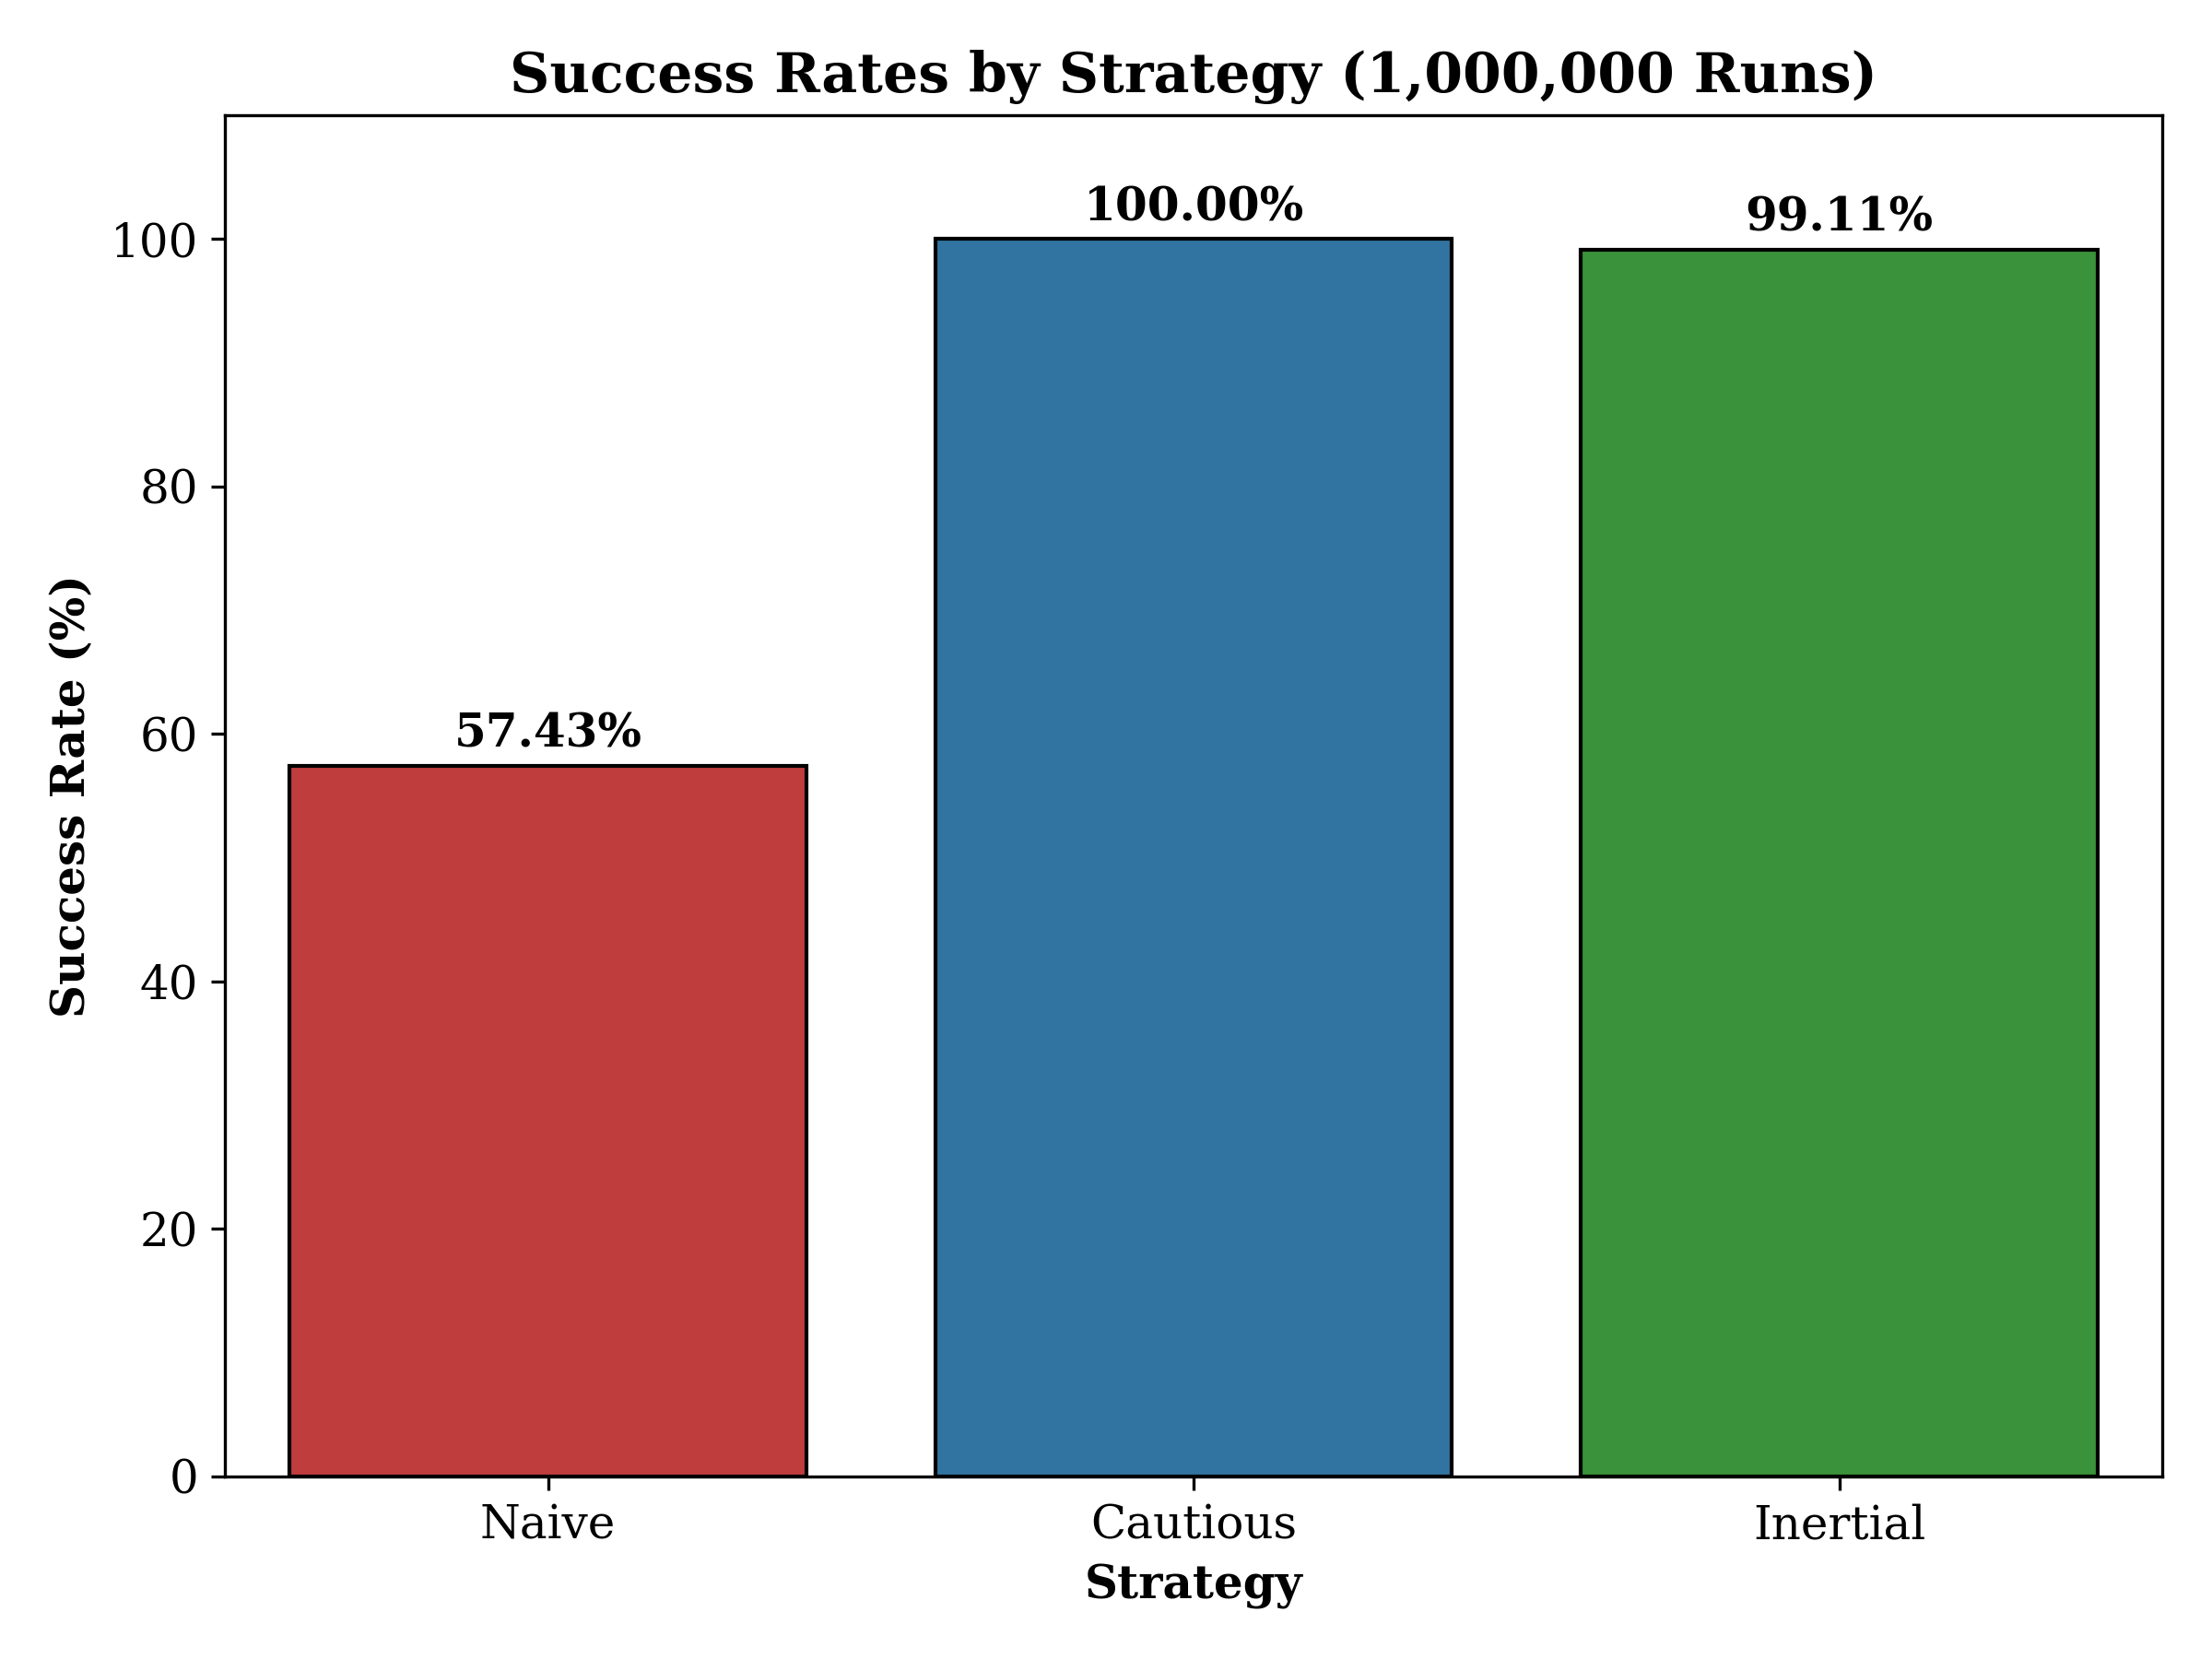
\includegraphics[height=4.5cm,keepaspectratio]{success_rates.png}
        \caption{Success rates of the Naive, Cautious, and Inertial strategies across $1{,}000{,}000$ randomized environments.}
        \label{fig:success_rates}
    \end{minipage}\hfill
    \begin{minipage}[t]{0.48\linewidth}
        \centering
        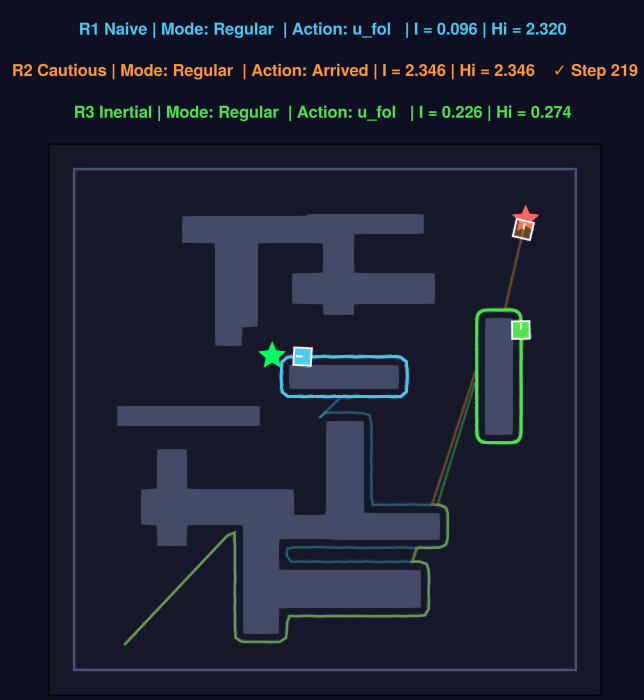
\includegraphics[height=4.5cm,keepaspectratio]{simulation_trap.png}
        \caption{Visualization of the cyclic synchronization trap. The Inertial robot (green) enters an infinite boundary-following loop due to open-loop motion during spoofing, while the Cautious robot (orange) breaks the cycle by pausing.}
        \label{fig:sim_trap}
    \end{minipage}
\end{figure}

\section{Conclusion and Limitations}
A temporal filter can protect I-Bug from sufficiently abrupt additive spoofing without odometry. Cautious preserves the nominal path and, under finite cumulative interference, inherits nominal convergence; Inertial is faster in the reported simulations but is not guaranteed to converge. The guarantee does not cover gradual ramping attacks, transitions below the detection threshold, unbounded interference, or model mismatch in $K$, $v_{\max}$, and the noise margin. Future work will address adaptive thresholds, spatial adversarial fields, and hardware experiments.

\begin{thebibliography}{9}
\small

\bibitem{taylor2009}
K.~Taylor and S.~M. LaValle,
``I-Bug: An intensity-based bug algorithm,''
in \emph{Proc. IEEE International Conference on Robotics and Automation}, 2009.

\bibitem{taylor2014}
K.~Taylor and S.~M. LaValle,
``Intensity-based navigation with global guarantees,''
\emph{Autonomous Robots}, 2014.
\end{thebibliography}

\end{document}	